\documentclass[12pt]{report}
\pagestyle{plain}

%\usepackage{subfigure}
\usepackage{cancel}
\usepackage{setspace}
\usepackage{biblatex}
\usepackage{amssymb,graphicx,color}
\usepackage{amsfonts}
\usepackage{latexsym}
\usepackage{a4wide}
\usepackage{amsmath}
\usepackage{csvsimple}
\usepackage[utf8]{inputenc}
\usepackage{todonotes}
\usepackage{bigints}
\usepackage{hyperref}

\allowdisplaybreaks

\hypersetup {
    hidelinks
}

\addbibresource{references.bib}

\newtheorem{theorem}{THEOREM}
\newtheorem{lemma}[theorem]{LEMMA}
\newtheorem{corollary}[theorem]{COROLLARY}
\newtheorem{proposition}[theorem]{PROPOSITION}
\newtheorem{remark}[theorem]{REMARK}
\newtheorem{definition}[theorem]{DEFINITION}
\newtheorem{fact}[theorem]{FACT}

\newtheorem{problem}[theorem]{PROBLEM}
\newtheorem{exercise}[theorem]{EXERCISE}
\def \set#1{\{#1\} }

\newenvironment{proof}{
PROOF:
\begin{quotation}}{
$\Box$ \end{quotation}}


\DeclareMathOperator{\EX}{\mathbb{E}}% expected value
\DeclareMathOperator{\VAR}{\mathbb{V}}% expected value
\DeclareMathOperator*{\argmin}{arg\,min}
\DeclareMathOperator*{\argmax}{arg\,max}

\newcommand{\bs}{\boldsymbol}
\newcommand{\tb}{\textbf}
\newcommand{\pc}[2]{p(#1 \mid #2)}
\newcommand{\mc}[1]{\mathcal{#1}}
\newcommand{\mb}[1]{\mathbb{#1}}
\newcommand{\half}{\frac{1}{2}}
\newcommand{\E}{\mathbb{E}}
\newcommand{\inv}[1]{#1^{-1}}
\newcommand{\sumlim}[3]{\sum\limits_{#1 = #2}^{#3}}
\newcommand{\suml}[1]{\sum\limits_{#1}}
\newcommand{\prodlim}[3]{\prod\limits_{#1 = #2}^{#3}}
\newcommand{\prodl}[1]{\prod\limits_{#1}}
\newcommand{\ub}{\underbrace}
\newcommand{\intlim}[2]{\int\limits_{#1}^{#2}}
\newcommand{\diff}[1]{\frac{d}{d#1}}
\newcommand{\prl}{\partial}
\newcommand{\ol}{\overline}
\newcommand{\argminl}[1]{\argmin\limits_{#1}^{}}
\newcommand{\argmaxl}[1]{\argmax\limits_{#1}^{}}
\newcommand{\comb}[2]{\begin{pmatrix}#1 \\ #2\end{pmatrix}}

\renewcommand{\P}{\mathbb{P}}
\renewcommand{\bs}{\boldsymbol}

%%%%%%%%%%%%%%%%%%%%%%%%%%

\title{  	{ 
\includegraphics[scale=.5]{ucl_logo.png}}\\
{{\Huge Inference In Random Geometric Graphs}}\\
		}
\date{Submission date: $11^\text{th}$ of September 2020}
\author{R\u{a}zvan - Dumitru Meriniuc\thanks{
{\bf Disclaimer:}
This report is submitted as part requirement for the Machine Learning MSc at UCL. It is
substantially the result of my own work except where explicitly indicated in the text.
The report may be freely copied and distributed provided the source is explicitly acknowledged.}
\\ \\
Machine Learning MSc\\ \\
Peter Orbanz}

\doublespacing
\begin{document}
 
\maketitle
\begin{abstract}
    The graph is a ubiquitous data structure, arising in numerous real-world scenarious, ranging from social networks to drug design. While relatively simple, it is difficult to exploit it in the context of machine learning, which prompts one to find ways of encoding it in a geometric space with a well-defined metric. Our work aims to study how feasible it is to treat the embeddings of the nodes of a graph as latent variables, in the context of random geometric graphs (RGG) and Bayesian statistics. By placing a prior on the embeddings and drawing an edge between two points randomly, based on the distance between them, we intent to approximate the posterior of the embeddings, given the graph, which would allow us to better describe the geometry capturing the properties of the graph.

\end{abstract}
\tableofcontents
\setcounter{page}{1}


\chapter{Introduction}
The graph is a ubiquitous data structure, which arises in numerous real-world scenarios, ranging from social networks to drug design. Its relative simplicity allows one to attach a myriad of semantics to the nodes and edges, hence its prevalence. However, its format limits the scope of machine learning techniques one can use on such data, but embedding its vertices in a geometry, be it euclidean or with a non-zero curvature, allows us to extend the range of methods we can use while modelling the data. This idea arises naturally, as many networks coming from physical considerations are governed by an underlying geometry, such as the road network in a country. \\

We are going to focus on data given as a simple homogeneous graph, i.e unweighted, undirected graph that contains no self-loops and no multiple edges\parencite{simplegraphdef}. The homogeneity refers to the edges representing the same concept. Mathematically, we define it as a pair $G = (V, E)$, where $V$ is the set of vertices, also called nodes, and $E$ is the set of edges. We will just represent the vertices as consecutive natural numbers, so $V = {1,\,2,\,\dots\,N}$, and the edges as unordered pairs $\{i,\, j\}$, $i \neq j$, $i,\,j \in V$. Such a graph can be completely defined by its adjacency matrix, $A$, $A_{ij} = 1$ if $\{i,\,j\} \in E$ and 0 otherwise, as we are working with unweighted edges, so we are interested whether an edge exists or not. Since the graphs is undirected, $A_{ij} = A_{ji}$. \\

The aim of this project is to study the latent geometric space in a Bayesian setting. The literature generally focuses on empirical embeddings (NLP), targetting the individual nodes, while we are more interested in the underlying geometry. A random geometric graph (RGG) is usually generated by sampling points from some space, representing the nodes, and connect each pair by an edge if the distance between them is less than some fixed threshold. In order to avoid this step function and the extra hyperparameter, we generate an edge stochastically, again relying on the distance between the points. The closer two points are, the greater the chance of them being connected. \\

In the literature, embeddings of nodes, edges and even whole subgraphs have been studied. We are going to focus on embedding of nodes only. They are generally studied from a graph theoretical or algorithmic point of view, the subject of embeddings in machine learning focusing more on how well they work for specific tasks and empirically determined. We aim, however, to describe in probabilistic terms the distribution of the embeddings and perform inference, which has not been studied so far, to our knowledge.

\chapter{Background And Related Work}

\section{Bayesian Statistics And Variational Inference}

We are going to work in the framework of Bayesian statistics, which relies on the Bayesian interpretation of probabilities, where the probability conveys the degree of belief in an event, which may rely on prior knowledge about the event, whether it is a personal belief or based on results of previous experiments. This is in contrast to the frequentist interpretation, which views probability as the limit of the relative frequency of an event after a great number of trials. \\

The cornerstone of Bayesian statistics is Bayes' formula. If $X$ is some data generated by a process with parameter $\theta$, then

\begin{definition}[Bayes' Formula, Posterior, Likelihood, Prior, Evidence]
\label{eq:bayesdef}
\begin{equation*}
    \mb{P}(\theta \mid X) = \frac{\mb{P}(X \mid \theta)\mb{P}(\theta)}{\mb{P}(X)}
\end{equation*}
\begin{enumerate}
    \item The \textbf{posterior} distribution, $\mathbb{P}(\theta \mid X)$, represents our updated belief about the parameter $\theta$ after observing the data $X$.
    \item The \textbf{likelihood} distribution, $\mathbb{P}(X \mid \theta)$, denotes the probability of the data being generated by the given the parameter $\theta$.
    \item The \textbf{Prior} distribution, $\mathbb{P}(\theta)$, quantifies our assumption about the parameter $\theta$.
    \item The \textbf{Evidence} distribution, $\mathbb{P}(X)$, represents the probability of the data occurring, which is computed by marginalising out the parameter $\theta$.
\end{enumerate}
\end{definition}

The central Bayesian principle consists of placing a probability over the parameters, thus giving rise to the prior. It is asymptotically equivalent to the frequentist method, the parameter converging to the true one, but the downside is that there is no mathematical decision theory one can rely on when choosing the prior. It is totally up to the practitioner, which allows us to insert our belief into the model, thus forcing us to be honest about the assumptions we make regarding the data and learning process. \\

Statistical inference is the process of using data analysis to deduce properties of an underlying probability distribution. For example, if we model some data according to a Gaussian distribution with a known variance, we can look at the data and infer what the mean is, and then use it to make predictions on new input points. When predicting, we could work with the parameter for which the data is most likely to occur, an estimate known as MAP (Maximum a posteriori), or average over the parameters in a Bayesian setting, by marginalisation, such that each element of the average has a weight represented by the posterior:

\begin{align}
    \mathbb{P}(\textbf{X*} \mid \textbf{X}) &= \int_{\Theta} \mathbb{P}(\textbf{X*}, \theta \mid \textbf{X}) d\theta = \int_{\Theta} \mathbb{P}(\textbf{X*} \mid \theta, \textbf{X}) \mathbb{P}(\theta \mid \textbf{X}) d\theta \\ 
    &= \int_{\Theta} \mathbb{P}(\textbf{X*} \mid \theta) \mathbb{P}(\theta \mid \textbf{X}) d\theta = \E_{\P(\theta \mid \bs{X})}[\P(\bs{X^*} \mid \theta)], \notag
\end{align}

\noindent
where $\textbf{X}$ is the observed data, $\textbf{X*}$ are the points for which we are trying to predict a quantity of interest, $\Theta$ is the parameter space and $\theta$ is an arbitrary parameter. $\P(\textbf{X*} \mid \theta, \textbf{X})$ becomes $\P(\textbf{X*} \mid \theta)$ because the model is fully specified given the parameters, the known points $\bs{X}$ adding no information. \\

\noindent
This integral requires a closed form of the posterior, which is often intractable because we cannot calculate the evidence present in the denominator in \textbf{Definition 1}, $\P(\bs{X})$. Even if it can be calculated, the posterior is not usually the probability density function a known distribution, which would make it more difficult to study and use. A possible solution would be to approximate it with the average $\frac{1}{N}\sum\limits_{i = 1}^N \P(\bs{X^*} \mid \theta_i)$, where $\{\theta_i\}_{i = 1}^N$ are the samples from $\P(\theta \mid \bs{X})$. The most popular class of sampling algorithms is Markov Chain Monte Carlo (MCMC) . For example, the Metropolis - Hastings algorithm allows us to circumvent the evidence, which cancels out. One of the drawbacks of this method is that it is non-deterministic and, in addition, we would not be able to measure how good our approximation is. Furthermore, there is the problem of choosing the hyperparameters, parameters of the model that are not governed by a prior, as they are just scalars whose value we need to determine. The classical approach aims to maximise the probability of the observed data, $\P(\bs{X})$, which is the term that generates the intractable integral preventing us from calculating the posterior in the first place. We could again employ sampling to address this issue, adding an extra layer of randomness to our implementation, which is undesirable. This technique we are about to present deals with the approximation of the posterior with a new variational distribution, offering a measure of \textit{distance} between the distributions, thus allowing us to determine how good our approximation is, which means that there is some quantity that tells us if we are working in the right direction. The setting of this approach offers a lower-bound of the evidence as a by-product, while we are making the approximation better, which is where the beauty of this method lies. While it does not provide a hard maximum for the evidence, we get the next best thing, a lower bound. \\

\noindent
The measure between distributions is called the Kullback - Leibler divergence , which is defined for any two distributions that share the support of the random variable.

\begin{definition}[Kullback - Liebler Divergence]
\begin{equation*}
    KL(q(u)\, ||\, \mathbb{P}(u)) = \int q(u) log \frac{q(u)}{\mathbb{P}(u)} du
\end{equation*}
\end{definition}
\noindent
Please note that this measure is asymmetric and, following Gibbs' inequality , non-negative , equalling 0 only when the two distributions are exactly the same. \\

\noindent
In our case, we would like to approximate the posterior $\P(\theta \mid \bs{X})$ with a new distribution $q(\theta)$, having free parameters, that would behave as if it has seen the data. The advantage is that we can pick whatever variational distribution we want, allowing us to insert extra assumptions that would make calculations easier. This means that we can keep the model \textit{pure} and add simplifications in the approximation. We would thus like to minimise the KL divergence between the two distributions. Because calculating it involves working with the original posterior, which posed problems from the beginning, we rely on the following result, which rephrases the problem as maximising a different term, directly implying the minimisation of our divergence.

\begin{align}
    log\mathbb{P}(\textbf{X}) &= KL(q(\theta) || \mathbb{P}(\theta \mid \textbf{X})) + \mc{F}(\theta) \\
    \mc{F}(\theta) &= \E_{q(\theta)}[log\mathbb{P}(\textbf{X}, \theta)] - H(q(\theta))
\end{align}
\noindent
where $H(q(\theta))$ is the entropy of the variational distribution and $\mc{F}$ stands for free energy, a concept coming from thermodynamics. This result is deduced in Appendix, section A.1. \\

\noindent
We can see how maximising $\mc{F}$ implies minimising the KL term. Because the divergence is non-negative, we get that
\begin{equation}
    log \P(\bs{X}) \geq \mc{F}(\theta)
\end{equation}
which acts as a lower bound for our evidence. Alternatively, we can deduce the same result, by-passing the KL term, using Jensen's inequality applied to the expected value, as shown in section A.1 of the Appendix.\\

\noindent
Please note that we have not yet touched the hyperparameters of either distribution. Assuming we could somehow compute $KL(q(\theta) || \P(\theta \mid \bs{X}))$ and pick the parameters that minimise it, it is not exactly obvious how doing this would provide a better chance for our data, expressed as a lower bound in our case, since it looks like this just gets the distributions closer disregarding the other terms. And this is the beauty of this technique. That striving for a better approximation generates a better lower bound for the data, addressing both aspects of the model that raised problems, mentioned at the beginning of this section. In practice, we optimise both sets of hyperparameters at the same time to maximise $\mc{F}$, which we should be able to compute effectively. We choose the variational distribution $q$, so we ought to get a closed form of its entropy, while $log \P(\bs{X}, \theta)$ is the model itself, and if we cannot express it, then we know nothing. Thus, we transform this Bayesian inference problem into an optimisation one. \\

\noindent
In some cases, such as the model we are proposing in \textbf{Chapter 3}, we run into terms of the free energy we cannot calculate and have to rely on approximations through sampling. While not ideal, this is done in the same setting and we can still measure how good our approximation of the posterior is, albeit this \textit{distance} is just an estimate as well. \\

\noindent
Prediction is performed by approximating $\P(\theta \mid \bs{X})$ with $q(\theta)$ in the integral at (1.1), thus
\begin{equation}
    \E_{q(\theta)}[\P(\bs{X*} \mid \theta)] \approx \E_{\P(\theta \mid \bs{X})}[\P(\bs{X*} \mid \theta)]
\end{equation} \\

\section{Random Geometric Graphs}
The beginning of random graph theory is usually attributed to the publication of the seminal papers of Erd\H{o}s and R\'{e}nyi[reference] introducing the standard random graph model, which studies the behaviour of a random graph with n nodes and N edges, placing an uniform prior on all graphs that respect this requirement. However, around the same period of time, Gilbert [reference] proposed a different random graph model, which relies on a geometric layout underpinning the nodes, edges being determined based on the relative position of vertices. We are going to refer to the latter model by \textit{random geometric graph}. \\

A Poisson process was employed to model the geometric points, with the idea that they ought to be spread uniformly around the plane with a positive density. \\

\begin{definition}
    A Poisson process $\mc{P}$ with density one in $\mb{R}^2$ is a random subset of $\mb{R}^2$ such that:
    \begin{enumerate}
        \item The number of points in a measurable set A is governed by a Poisson distribution with the mean equal to the Lebesgue measure of A
        \item For two disjoint, measurable sets $A, B \subset \mb{R}^2$, the number of points they contain are independent from each other \\
    \end{enumerate}
\end{definition}

In the original model, points are picked in $\mb{R}^2$ according to a Poisson process with density one, connecting pairs of points if the distance between them is at most $R$. So, according to the first property of the definition above, the expected number of neighbours a point has is $N = \pi R^2$. A final version of this model can be constructed by restricting the space to a square of area $n$, ensuring the number of points, which is a Poisson random variable, has average $n$. There are many results studying the asymptotic behaviour as $n \Rightarrow \infty$ and algorithms to recover points with a certain error (reference paper found). Spherical RGG and Erdos [paper?].\\

Another level of randomness can be added, producing a \textit{soft random geometric graph}, which does not rely on a threshold value, but uses a connection function, $\phi$, which takes as a parameter the distance between two points, the output becoming the mean a Bernoulli random variable which determines the existence of an edge. This was introduced by Waxman [reference], using a stretched exponential, $\phi(d) = \beta e^{-\frac{d}{d_0}}$. This can be further generalised by introducing decay in the distance, $\phi(d) = \beta e^{-\left(\frac{d}{d_0}\right)^\eta}$. We have run experiments for $\eta \in \{1, 2\}$. \\

These structures have been mostly analysed in the context of graph theory, their asymptotic behaviour and connection to the Erd\H{o}s-R\'{e}nyi graph, and not in as determining the latent space for a graph in the context of inference in machine learning, to our knowledge, so this is what we aim to study.

\section{Exchangeability}
Is our model not Bayesian because the graphon is deterministic? \\

One can view statistical inference as the procedure of extracting a pattern, characterised as the parameter of the model, from observed data. This leads to understanding the randomness in the data source as the underlying pattern combined with the sample randomness. When such a common pattern exists and the data is not completely beclouded by the sample randomness, exchangeability properties supply criteria for when extracting the underlying patterns is possible. \\

In practice, when working with a model in a Bayesian manner, we usually make use of Bayes' formula in the following form 

\begin{definition}[Bayes' Formula, Posterior, Likelihood, Prior, Evidence]
\label{eq:bayesdef}
\begin{equation*}
    \mathbb{P}(d\theta \mid X_{1:N}) \overset{a.s.}{=} \frac{\prodlim{i}{1}{N}p_\theta(x_i)}{\bigintsss\limits_{\bs{T}}\prodlim{i}{1}{N}p_{\theta'}(x_i)\mb{P}(d\theta')}\mb{P}(d\theta)
\end{equation*}
where $\mb{P}$ is a prior distribution, $\bs{T}$ is the parameter space of $\theta$, $p_\theta$ is a probability density function and $X_{1:N}$ represents N observations.
\end{definition}

We make considerable assumptions, which consist not only of the choice of likelihood density and prior distribution, but also that, given a parameter $\theta$ from the random variable $\Theta$, the joint likelihood of the observations factorises, so

\begin{equation}
    p_\theta(x_1,\,\dots\,,x_N) = \prodlim{i}{1}{N}p_\theta(x_i)
\end{equation}

Our assumption is that the observations $X_1,\,\dots,\,X_N$ independent and identically distributed given $\Theta$, which makes them \textbf{conditionally independent}. We can mathematically express that as
\begin{equation}
    \mb{P}(X_{1:N} \in dx_1 \times\dots\times dx_N \mid \Theta) \overset{a.s.}{=} \prodlim{i}{1}{N}\mb{P}(X_i \in dx_i \mid \Theta)
\end{equation}

This assumption of conditional independence sits at the core of Bayesian modelling, implying that, given $\Theta$, the randomness attributed to the observations decouples entirely, so all the joint information in the sampled data is enclosed in $\Theta$, which becomes our quantity of interest we would like to extract from the observations. Exchangeability then seeks to provide the context in which we may assume that conditional independence, given some random quantity, is met. \\

\begin{definition}[Exchangeability]
    A random sequence $X_{1:\infty} = (X_1,\,X_2,\,\dots\,)$ is said to be \textbf{exchangeable} if the order in which the values $X_i$ are observed is irrelevant to their joint distribution. Mathematically, we write this as
    \begin{equation}
        (X_1,\,X_2,\,\dots) \overset{d}{=} (X_{\pi(1)},\,X_{\pi(2)}\,\dots),\quad \forall \text{bijections } \pi : \mb{N} \rightarrow \mb{N}
    \end{equation}
\end{definition}

We can see that an i.i.d. sequence is obviously exchageable, since their distribution is a product, which commutes. The same holds for a conditionally i.i.d. sequence, given some $\Theta$, since it is a product like in (2.8), so the set of conditionally i.i.d. sequences is contained in the set of exchageable sequences. The seminal result by de Finetti surprisingly proves that these two sets are actually equal, so a sequence $X_{1:\infty}$ is exchangeable if and only if it is conditionally i.i.d, for some $\Theta$. \\

Defining $P_\theta(\bullet) := \mb{P}(X_i \in \bullet \mid \Theta = \theta)$, we have a family of measures
\begin{equation}
    M := \{P_\theta \mid \theta \in \bs{T}\}
\end{equation}

Because $\Theta$ is random, $P_\Theta$ is a random varible in the set of all probability measures on the sample space $\bs{X}$, \textbf{PM(X)}, thus a random probability measure. Instead of thinking about $\Theta$ as a random parameter for the distribution governing our sequence, we may view it as a random probability measure, so \textbf{T} = \textbf{PM}(\textbf{X}), so that $P_\theta = \theta$. Abbreviating the factorial distribution as

\begin{equation}
    P_\theta^\infty(dx_1 \times dx_2 \dots) = \prod\limits_{i \in \mb{N}} P_\theta(dx_i)
\end{equation}
Let us now introduce de Finetti's Theorem.

\begin{theorem}[de Finetti]
    An infinite random sequence $X_{1:\infty}$ is exchangeable if and only if there exists a random probability measure $\Theta$ on $\bs{X}$, such that
    \begin{equation}
        \mb{P}(X_{1:\infty} \in \bullet \mid \Theta) \overset{a.s.}{=} \Theta^\infty(\bullet)
    \end{equation}
\end{theorem}

The theorem usually appears in the form below, which is a direct consequence of eq above, obtained by marginalising out the random probability measure $\Theta$, leading to equality in expectation only. We have that exchangeability implies eq below, but not the other way around. The right-hand side of the equation below is a mixture, which means that it can be sampled in two stages, by first generating $\Theta \sim \eta$ and then sampling $X_{1:N} \mid \Theta$ from $\Theta^\infty$, making $X_{1:\infty}$ condtionally i.i.d., which are already exchangeably. \\

\begin{corollary}
    A random sequence $X$ is exchangeable if and only if 
    \begin{equation}
        \mb{P}(X \in \bullet) = \int\limits_{\bs{P}\bs{M}(\bs{X})} \theta^\infty(\bullet) \eta(d\theta)
    \end{equation}
    for some distribution $\eta$ on \textbf{PM}(\textbf{X}).
\end{corollary}

We can alternatively present de Finetti's theorem using random variables instead of distributions. For $\theta \in$ \textbf{PM}(\textbf{X}) a probability measure on \textbf{X}, we denote the i.i.d. random sequence sampled from $\theta$ as
\begin{equation*}
    X_\theta^0 := (X_1, X_2,\dots),\quad\text{where}\, X_1, X_2,\dots \overset{i.i.d}{\sim} \theta
\end{equation*}
so $\mb{P}(X_\theta^0) = \theta^\infty$. Exchangeability is obtained by randomising $\theta$, i.e. if $\Theta$ is a random probability measure on \textbf{X}, then $X_\Theta^0$ is an exchangeable sequence. de Finetti's theorem is then restated as
\begin{equation}
    X_{1:\infty}\, \text{exchangeable}\, \Leftrightarrow X_{1:\infty} \overset{a.s.}{=} X_\Theta^0 \quad \text{for some}\, \Theta \in \bs{R}\bs{V}(\bs{P}\bs{M}(\bs{X}))
\end{equation}

This approach will be useful in expressing the more advanced representation theorems presented below, which can be presented more elegantly using random variables instead of distributions. \\

\subsection{Exchangeable Arrays}

A d-\textbf{array} is a type of structure defined as a potentially infinite collection of variables indexed by d indices,
\begin{equation}
    x := (x_{i_1,\,\dots,\,i_d})_{i_1,\,\dots,\,i_d \in \mb{N}},\quad \text{where} x_{i_1,\,\dots,\,i_d} \in \bs{X}_0
\end{equation}

The sequences previously discussed are 1-arrays and matrices can be seen as 2-arrays, with $\bs{X}_0$ an algebraic field, so that operations are well-defined. A simple graph, one with no multiple edges, can be represented by a 2-array, having $\bs{X}_0 = \{0, 1\}$, by its adjacency matrix. An undirected graph implies a symmetric matrix. We will continue to discuss only 2-arrays, but generalisations to generic d-arrays can be made as well (reference). \\

Let X be a random 2-array. We need to fix the components of X we are going to permute in order to define exchageability. Since the data is structured in rows and columns, it means that there is some semantic attributed to these sub-structures, otherwise we would just express the data as a regular sequence. Therefore, permuting should preserve the rows and columns, i.e. if two data points are located on the same column, they should still share that column after permuting them, regardless of the new order in which they appear, and similarly for rows. We thus reduce permutations of entries of X to permutations of its rows and columns, by either applying some permutation $\pi$ to both rows and columns, or use separate permutations, $\pi_r$ for rows and $\pi_c$ for columns.

\begin{definition}
    A random 2-array $X = (X_{ij})_{i,j \in \mb{N}}$ is said to be \textbf{jointly exchangeable} if
    \begin{equation}
        (X_{ij}) \overset{d}{=} (X_{\pi (i), \pi (j)}), \quad \forall\, \text{bijections}\,\pi:\mb{N} \rightarrow \mb{N}
    \end{equation}
    X is said to be \textbf{separately exchangeable} if
    \begin{equation}
        (X_{ij}) \overset{d}{=} (X_{\pi_r (i), \pi_c (j)}), \quad \forall\, \text{bijections}\,\pi_r, \,\pi_c:\mb{N} \rightarrow \mb{N}
    \end{equation}
\end{definition}

Peter figure \\

We can simply generate a random matrix by defining a function $f$ with its image equal to $\bs{X}_0$ and that has two arguments. Sampling two random sequences $(U_1,\,U_2,\,\dots)$ and $(V_1,\,V_2,\,\dots)$ and setting $X_{ij} := f(U_i, V_j)$ generates our random matrix. If the sequences $(U_i)$ and $(V_i)$ contain independent elements and are independent of each other, then $(X_{ij})$ is separately exchangeable. However, setting $X_{ij} := f(U_i, U_j)$, we generate a jointly exchangeable matrix. However, these are not all of the existing exchangeable arrays. We can, for example, add another argument to the function $f$, a random variable $U_{ij}$, without breaking the exchangeability, provided that the sequence $(U_{ij})$ is made of independent elements. The distributions governing the random variable we made use of is irrelevant, as they do not add any expressive power, so we are free to choose any convenient, simple distribution, such as the uniform distribution on $[0,\, 1]$. \\

\begin{definition}
    Let $\bs{F}(\bs{X}_0)$ be the space of measurable functions $\theta : [0,\,1]^3 \rightarrow \bs{X}_0$, $(U_i)$ and $(V_i)$ two i.i.d. sequences and $(U_{ij})$ an i.i.d. 2-array, all elements being Uniform[0,\,1] random variables. We define two random arrays, $J_\theta^0$ and $S_\theta^0$, for any $\theta \in \bs{F}$, as
    \begin{align}
        J_\theta^0 &:= \theta(U_i, U_j, U_{ij}) \\
        S_\theta^0 &:= \theta(U_i, V_j, U_{ij})
    \end{align}
\end{definition}

Incredibly, these two random arrays play an analogous role to that of i.i.d. sequences, in that any exchageable array can be generated by making $\theta$ random, result proven by Aldous and Hoover. \\

\begin{theorem}{Aldous, Hoover}
    A random 2-array $X = (X_{ij})$ with entries in a Polish space $\bs{X}_0$ is jointly exchangeable if and only if
    \begin{equation}
        X \overset{d}{=} J_\Theta^0,\quad \text{for some}\, \Theta \in \bs{RV}(\bs{F}(\bs{X}_0))
    \end{equation}
and separately exchangeable if and only if
    \begin{equation}
        X \overset{d}{=} S_\Theta^0,\quad \text{for some}\, \Theta \in \bs{RV}(\bs{F}(\bs{X}_0))
    \end{equation}
\end{theorem}

\begin{definition}
    A \textbf{graphon} is a measurable function $w : [0,\,1]^2 \rightarrow [0, 1]$.
\end{definition}

Its connection to exchangeable graphs arises when considering a symmetric adjacency matrix, thus working with simple, undirected graphs, as we can replace the three-argument function $\theta$ in $J_\theta^0$ with our graphon $w$, which only takes two arguments. For $\theta \in \Theta(\{0, 1\})$ and a uniform random variable U, $\theta(x, y, U) \in \{0,\,1\}$, so we can define $w$ as
\begin{equation}
    w(x, y) := \mb{P}[\theta(x, y, U) = 1]
\end{equation}
which makes it a measurable function $[0,\,1]^2 \rightarrow [0,\,1]$. For a fixed $w$, we can sample a random graph $G_w^0$ as follows:
\begin{align}
\begin{split}
    U_1,\,U_2,\,\dots &\overset{iid}{\sim} Uniform[0, 1] \\
    X_{ij} &\sim Bernoulli(w(U_i,\,U_j))
\end{split}
\end{align}

\section{Quadratic Forms In Random Variables}
For a random variable of dimension $n$, $X \sim \mc{N}(\bs{\mu}, \Sigma)$, we are interested in finding the probability distribution function of the quadratic form $Q = X^TX$. When our embeddings are governed by a multivariate Gaussian distribution, their difference will also be a multivariate Gaussian random variable, so the aforementioned $Q$ represents the squared difference between two such i.i.d. embeddings. \\

Theorem 4.2b.1 in Mathai states that the density we are looking for is
\begin{equation}
    f(u) = \sumlim{k}{0}{\infty}(-1)^kc_k\frac{u^{\frac{n}{2} + k - 1}}{\Gamma(\frac{n}{2} + k)},\quad 0 < u < \infty
\end{equation}
where
\begin{align}
    c_0 &= \text{exp}\left(-\half\sumlim{j}{1}{n}b_j^2\right)\prodlim{j}{1}{n}(2\lambda_j)^{-\half} \\
    c_k &= \frac{1}{k}\sumlim{r}{0}{k - 1}d_{k-1}c_r,\quad k \leq 1 \\
    d_k &= \half\sumlim{j}{1}{n}(1 - kb_j^2)(2\lambda_j)^{-k},\quad k \leq 1 \\
\end{align}
with $\lambda_j$ being the $j^\text{th}$ eigenvalue of $\Sigma$ and $\bs{b} = P\Sigma^{-\half}\bs{\mu}$, where $P$ is the matrix with its columns equal to the eigenvectors corresponding to the eigenvalues $\{\lambda\}$, so
\begin{equation}
    P^T\Sigma P = \text{diag}(\lambda_1,\,\dots,\,\lambda_n)
\end{equation}

More on this can be found in Mathai, chapters 3 and 4.

\chapter{RGG Inference}
Let us denote the given data by $\mc{G} = \{X_{ij}\}_{i, j \in [N]}$, where $X_{ij} \in \{0,1\}$ represents the existence of an edge between nodes $i$ and $j$, assuming nothing that would induce and structure in the given graph. We model this data as arising from an SRGG, with the embeddings governed by an underlying Gaussian distribution. Let $X_i \in \mb{R}^n$ denote the embedding of vertex $i$. The random variable representing an edge, $X_{ij}$ is then a Bernoulli random variable, with mean $e^{-\text{dist}(X_i, X_j)^2}$.\todo{Use distance only -> Chi Distribution} \\

Assume the prior embeddings are generated by a multivariate Gaussian with mean $\bf{0}$, which is chosen to facillitate calculations, but is otherwise irrelevant, since the distance between points ignores the global position of the points, and covariance matrix $\mc{I}$. We are interested in approximating the posterior $\mb{P}(\bs{X} \mid \mc{G}),\, \bs{X} = \{X_i\}_{i \in [N]}$ by a known distribution, a multivariate Gaussian with mean $\bs{0}$ and covariance matrix $\sigma^2\mc{I}$, where $\sigma$ is a hyperparameter. We thus make use of an approximating distribution $q$,
\begin{align*}
    q(\bs{X}) &\approx \mb{P}(\bs{X} \mid \mc{G}) \\
    \bs{X} &\overset{q}{\sim} \mc{N}(\bs{0}, \sigma^2\mc{I})
\end{align*}

Working in a variational inference setting, we aim to find the hyperparameters tha maximise the free energy
\begin{align*}
    \mc{F}(\sigma) = \left<log\mb{P}(\mc{G} \mid \bs{X})\right>_{q(\bs{X})} - KL[q(\bs{X}) \mid\mid \mb{P}(\bs{X} \mid \mc{G})] \\
\end{align*}

Le us focus on the first term for now, denoting the value of the square distance between two Gaussian embeddings by $u_{ij} = \text{dist}(X_i, X_j)^2$, and capitalising it to represent the random variable associated with it.
\begin{align*}
    \left<log\mb{P}(\mc{G} \mid \bs{X})\right>_{q(\bs{X})} &= \int\limits_{(\mb{R}^n)^N} q(\bs{X})log\mb{P}(\mc{G} \mid \bs{X}) d\bs{X} \\
    &= \int\limits_{(\mb{R}^n)^N} q(\bs{X}) \prodl{i<j} e^{-u_{ij}X_{ij}}(1 - e^{-u_{ij}})^{1 - X_{ij}} \\
    &= \suml{i<j}\int\limits_{(\mb{R}_{>0})^\frac{N(N-1)}{2}} q(\bs{U}) (-u_{ij}X_{ij} + (1 - X_{ij})log(1 - e^{-u_{ij}})) d\bs{U} \\
    &= \suml{i<j}\int\limits_{\mb{R}_{>0}} q(u_{ij}) (-u_{ij}X_{ij} + (1 - X_{ij})log(1 - e^{-u_{ij}})) du_{ij} \\
    &= \suml{i<j}\int\limits_{\mb{R}_{>0}} q(u_{ij}) \left(-u_{ij}X_{ij} + (1 - X_{ij})log\frac{e^{u_{ij}} - 1}{e^{u_{ij}}}\right) du_{ij} \\
    &= \suml{i<j}\int\limits_{\mb{R}_{>0}} q(u_{ij}) (-u_{ij}X_{ij} - (1 - X_{ij})u_{ij} + (1 - X_{ij})log(e^{u_{ij}} - 1)) du_{ij} \\
    &= \suml{i<j}\int\limits_{\mb{R}_{>0}} q(u_{ij}) (-u_{ij} + (1 - X_{ij})log(e^{u_{ij}} - 1)) du_{ij} \\
    &= -\comb{N}{2}<u>_{q(u)} + \suml{i<j}(1 - X_{ij})\int\limits_{\mb{R}_{>0}} q(u_{ij}) log(e^{u_{ij}} - 1) du_{ij} \\
    &= -\comb{N}{2}<u>_{q(u)} + \left(\comb{N}{2} - \ub{E}_{\text{\#edges}}\right)\int\limits_{\mb{R}_{>0}} q(u) log(e^{u} - 1) du
\end{align*}

Using that
\begin{equation*}
    q(u) = \frac{u^{m-1}(2\sigma^2)^{-m}}{(m-1)!}exp(-(2\sigma^2)^{-1}u)
\end{equation*}
we have
\begin{align*}
    \left<log\mb{P}(\mc{G} \mid \bs{X})\right>_{q(\bs{X})} &= -\comb{N}{2}2m\sigma^2 + \left(\comb{N}{2} - E\right)\frac{(2\sigma^2)^{-m}}{(m-1)!}\int\limits_{\mb{R}_{>0}} u^{m-1}exp(-(2\sigma^2)^{-1}u) log(e^{u} - 1) du
\end{align*}

The integral does not have a closed form, so we are forced to approximate it. Using the well-known result for the KL divergence between two multivariate Gaussians and that it is additive for independent distributions, we have that the free energy is

\begin{align*}
    \mc{F}(\sigma) &= -\comb{N}{2}2m\sigma^2 + \left(\comb{N}{2} - E\right)\frac{(2\sigma^2)^{-m}}{(m-1)!}\int\limits_{\mb{R}_{>0}} u^{m-1}exp(-(2\sigma^2)^{-1}u) log(e^{u} - 1) du \\
    &- Nm(-log(\sigma^2) - 1 + \sigma^2) \\
\end{align*}

\subsection{Relation To Graphons}
Due to a special case of the Borel isomorphism theorem, we are able to map a Uniform[0, 1] random variable to a multivariate Gaussian, which allows us to work with the latter when generating graphs, as per definition (?). Let $\phi : [0,\,1] \rightarrow \mb{R}^n$ be that mapping. If we work with the squared distance between embeddings to randomly determine the existence of an edge, the graphon we are working with is
\begin{equation}
    w(x, y) = e^{(\phi (x) - \phi (y))^T\phi (x) - \phi (y))}
\end{equation}

\section{Spherical RGG}
We can also model the embeddings as sitting on a hypersphere. We then have two possible approaches to measuring the geodesic, the shortest path between two points:
\begin{enumerate}
    \item In a spherical geometry, where the edges are curves on the sphere
    \item In a Euclidean setting, so the edges go through the sphere
\end{enumerate}

In both frameworks, we need to place a prior over the embedding points. Let us assume we are working with a unit-radius hypersphere, though nothing much changes when working with an arbitrary radius. The simplest distribution would be the uniform one, but that is not interesting enough, so we opt for the von Mises - Fisher distribution, which is akin to the normal distribution, except the points all have a fixed radius. Its probability density function is

\begin{equation}
    f_n(\bs{x}; \bs{\mu}, \kappa) = C_n(\kappa) e^{\kappa \bs{\mu}^T \bs{x}}
\end{equation}
where $\kappa > 0$ is the concentration parameter of the distribution around the mean direction $\bs{\mu}$, $\lVert \bs{\mu} \rVert = 1$. The greater $\kappa$ is, the more concentrated the points are, with $\kappa = 0$ determining a uniform distribution. The normalisation constant $C_n(\kappa)$ is
\begin{equation}
    C_n(\kappa) = \frac{\kappa^{\frac{n}{2} - 1}}{(2\pi)^{\frac{n}{2}}I_{\frac{n}{2} - 1}(\kappa)}
\end{equation}
where $I_u$ represents the modified Bessel function of the first kind at order $u$. \\

Since only the relative position of the points matters, we can pick any mean direction $\bs{\mu}$, so we can simplify our work by choosing $\bs{\mu} = (1,\,0,\,\dots,\,0)$, leaving only $\kappa$ to vary. We need to find the probability distribution function for the distance between two points governed by a von Mises - Fisher distribution. In the first framework, the distance between two points $\bs{x}_1$ and $\bs{x}_2$ is given by
\begin{equation}
    d = cos^{-1}(\bs{x}_1^T\bs{x}_2)
\end{equation}

\section{Hyperbolic RGG}

\chapter{Summary and Conclusion}
In this thesis, we study the potential of using random vertex embeddings as latent variables for a given adjacency matrix, working in the framework of random geometric graphs. We investigated Euclidean, spherical and hyperbolic spaces and relied on Bayesian variational inference to determine the posterior of the embeddings, given a graph. \\

The most challenging aspect of this work was the form of the probability density function for the distance between pairs of embeddings, which forced us to make assumptions that severly limited our model. Even for something as simple as a spherical multivariate Gaussian prior, we run into an intractable integral and the right parameters are not recovered for simple data. It gets even more complicated when placing the embeddings on the unit sphere or in a hyperbolic space, with little hope of generating sensible results when considering random variables for distances. \\

We assert that this avenue should be avoided.


\centering
\begin{table}
    \centering
    \tiny
    \csvautotabular{gaussian_mixture_again_m1.csv}
    \caption{Mixture of two Gaussians, centered at $\mu_1 = (0, 0)$ and $\mu = (2, 2)$, with covariance matrices $1.5\mc{I}$ and $\mc{I}$.}
\end{table}

\centering
\begin{table}
    \centering
    \tiny
    \csvautotabular{gaussian_mixture_again_far_m1.csv}
    \caption{Mixture of two Gaussians, centered at $\mu_1 = (0, 0)$ and $\mu = (7, 7)$, with covariance matrices $1.5\mc{I}$ and $\mc{I}$.}
\end{table}

\centering
\begin{table}
    \centering
    \tiny
    \csvautotabular{multivariate_t_15deg_spherical_again_m1.csv}
    \caption{Spherical Multivariate T with $\sigma$ given in the params column}
\end{table}

\begin{table}
    \centering
    \tiny
    \csvautotabular{gaussian_spherical_again_m1.csv}
    \caption{Spherical Gaussian with $\sigma$ given in the params column}
\end{table}

\centering
\begin{table}
    \centering
    \tiny
    \csvautotabular{gaussian_non_diag_again_m1.csv}
    \caption[Gaussian with non-diagonal covariance matrix]{Gaussian with covariance matrix $\begin{pmatrix} 3 & 1.5 \\ 1.5 & 1 \end{pmatrix}$ }
\end{table}

\centering
\begin{table}
    \centering
    \tiny
    \csvautotabular{multivariate_t_5deg_non_diag_again_m1.csv}
    \caption[Multivariate T with non-diagonal covariance matrix]{Multivariate T with 5 degrees of freedom and covariance matrix $\begin{pmatrix} 3 & 1.5 \\ 1.5 & 1 \end{pmatrix}$ }
\end{table}

\centering
\begin{table}
    \centering
    \tiny
    \csvautotabular{gaussian_ms.csv}
    \caption[Multiple ms]{Gaussian with identity covariance matrix for different ms.}
\end{table}

\begin{figure}
    \centering
    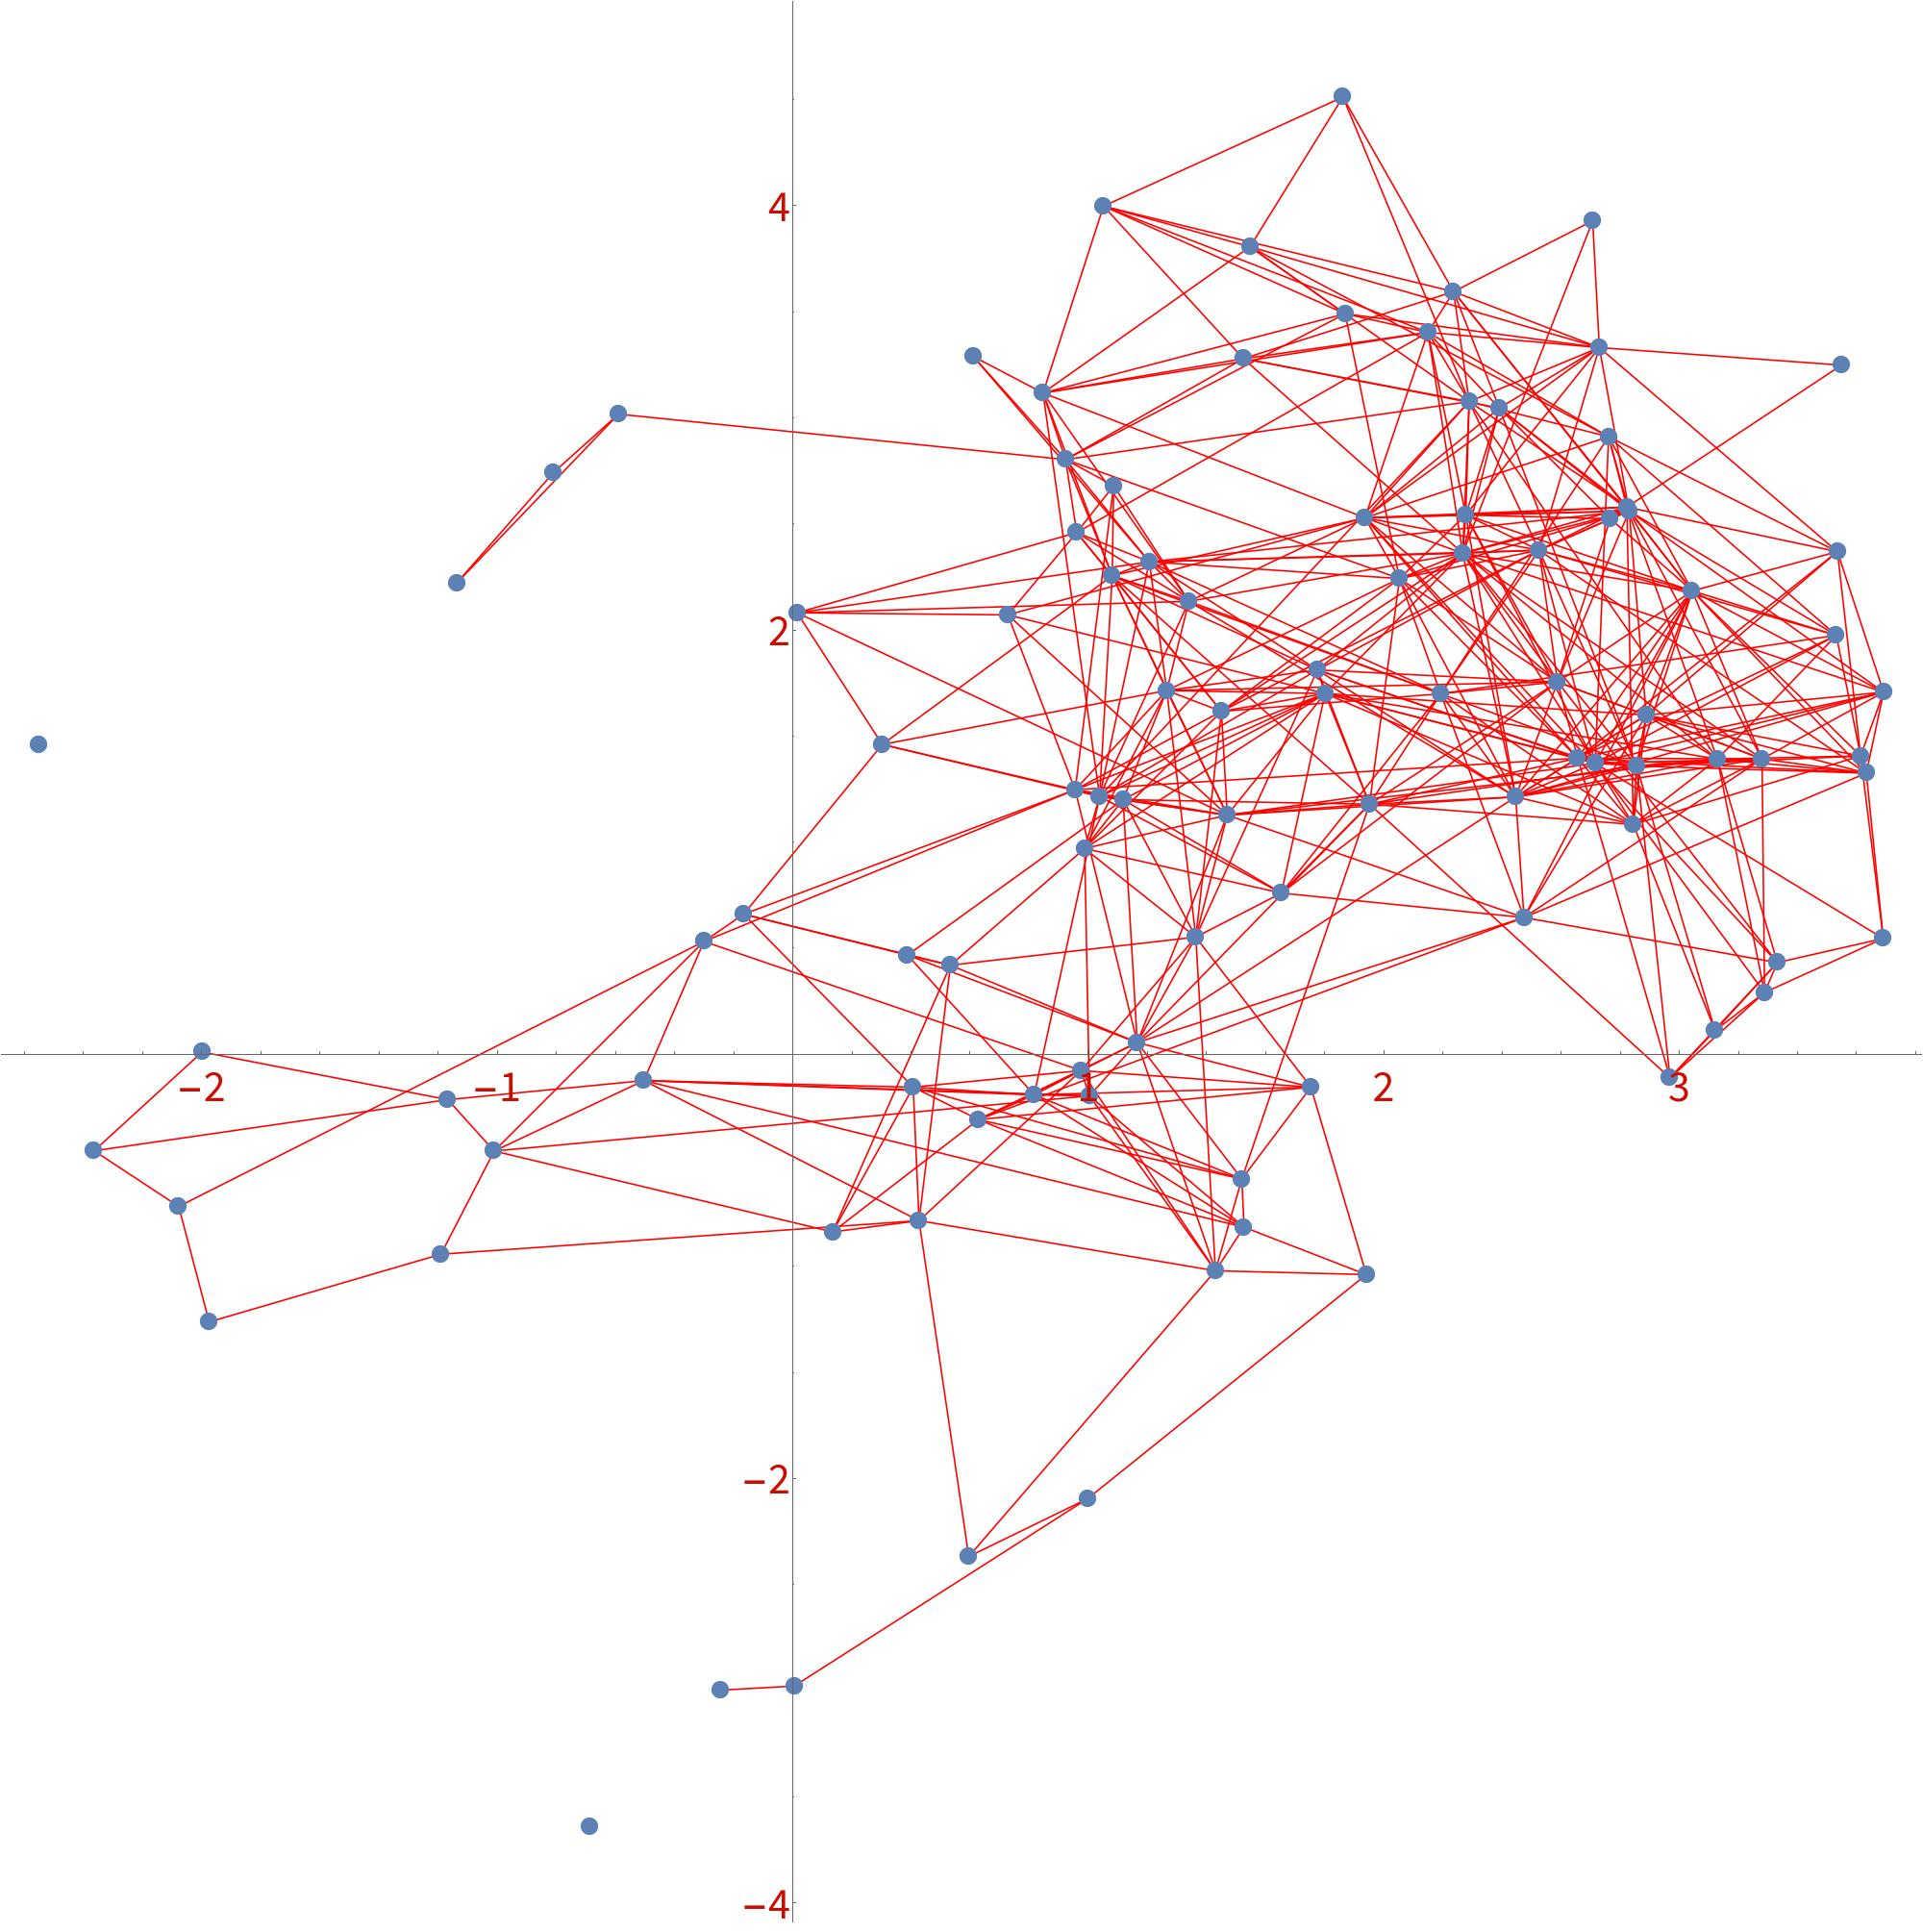
\includegraphics[width = 0.5\textwidth]{gaussian_mixtures.jpg}
    \caption{Mixture of two Gaussians, $\mu_1 = (0, 0),\, \mu_2 = (2, 2)$, $\Sigma_1 = 1.5\mc{I},\, \Sigma_2 = \mc{I}$, $\mb{\pi} = (0.4, 0.6)$}
\end{figure}

\begin{figure}
    \centering
    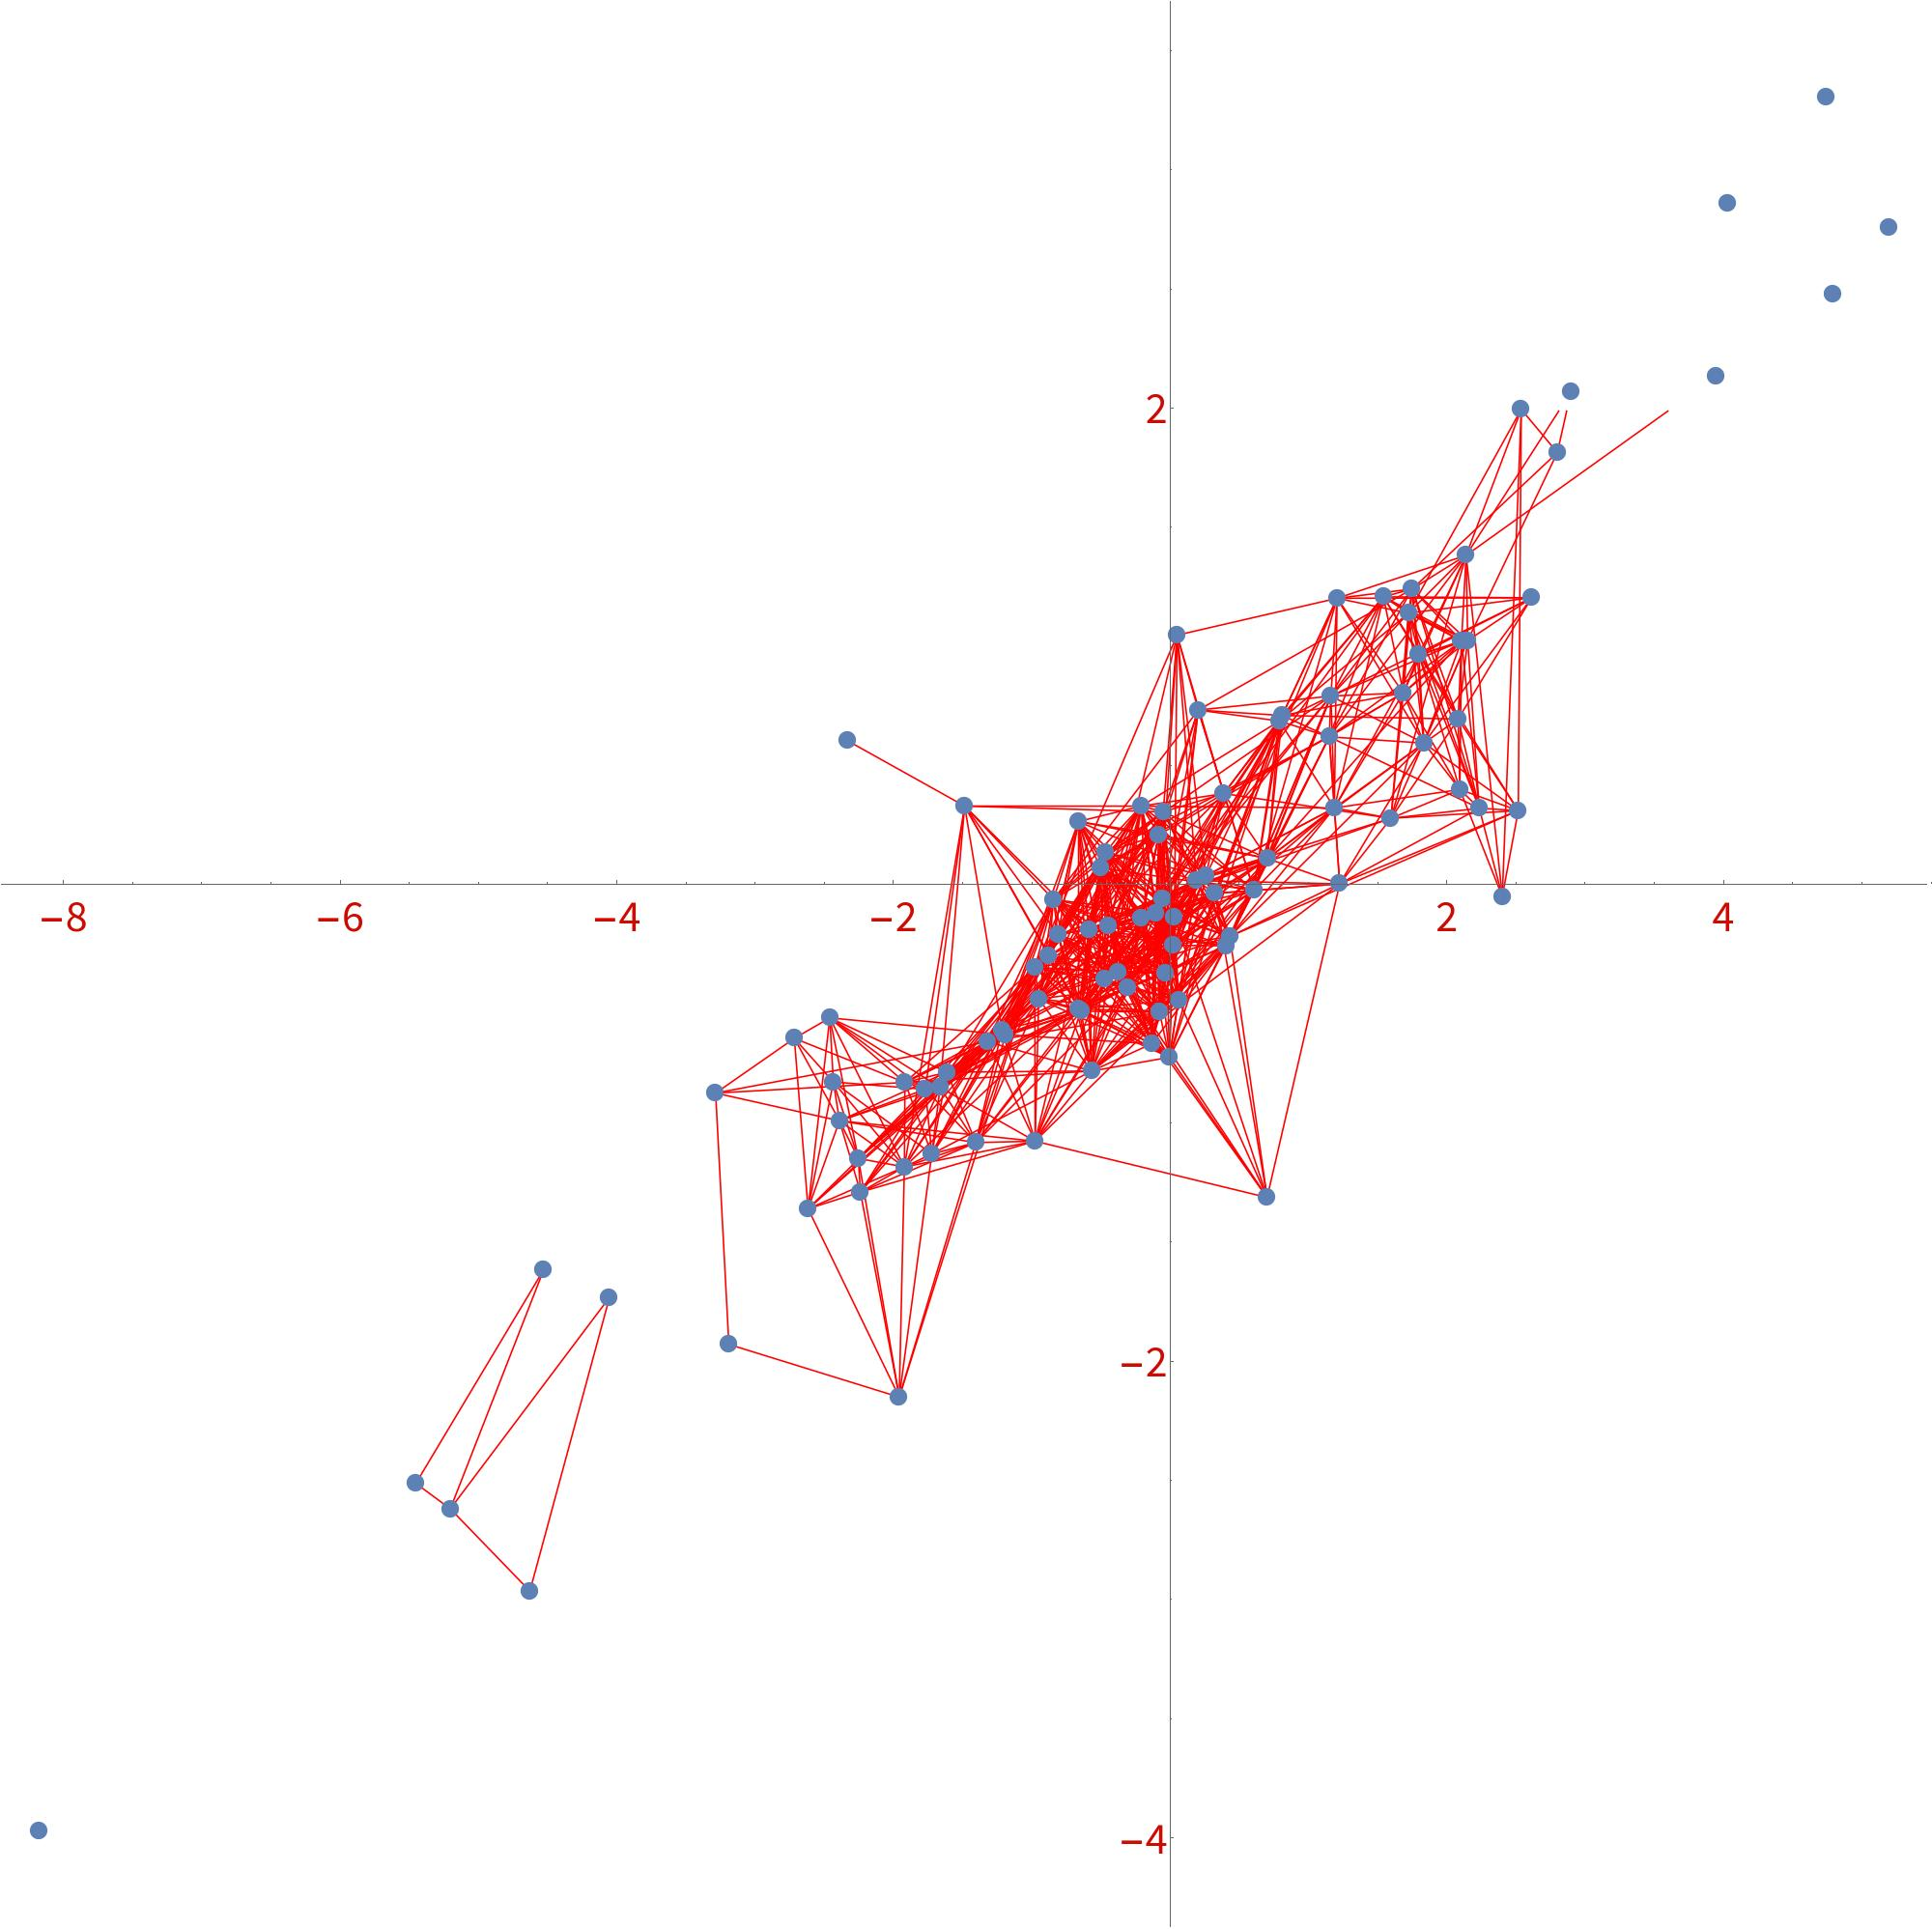
\includegraphics[width = 0.5\textwidth]{multivariatet_non_diag.jpg}
    \caption[Multivariate T]{Multivariate T with $\Sigma = \begin{pmatrix} 3 & 1.5 \\ 1.5 & 1\end{pmatrix}$ and 5 degrees of freedom.}
\end{figure}

\begin{figure}
    \centering
    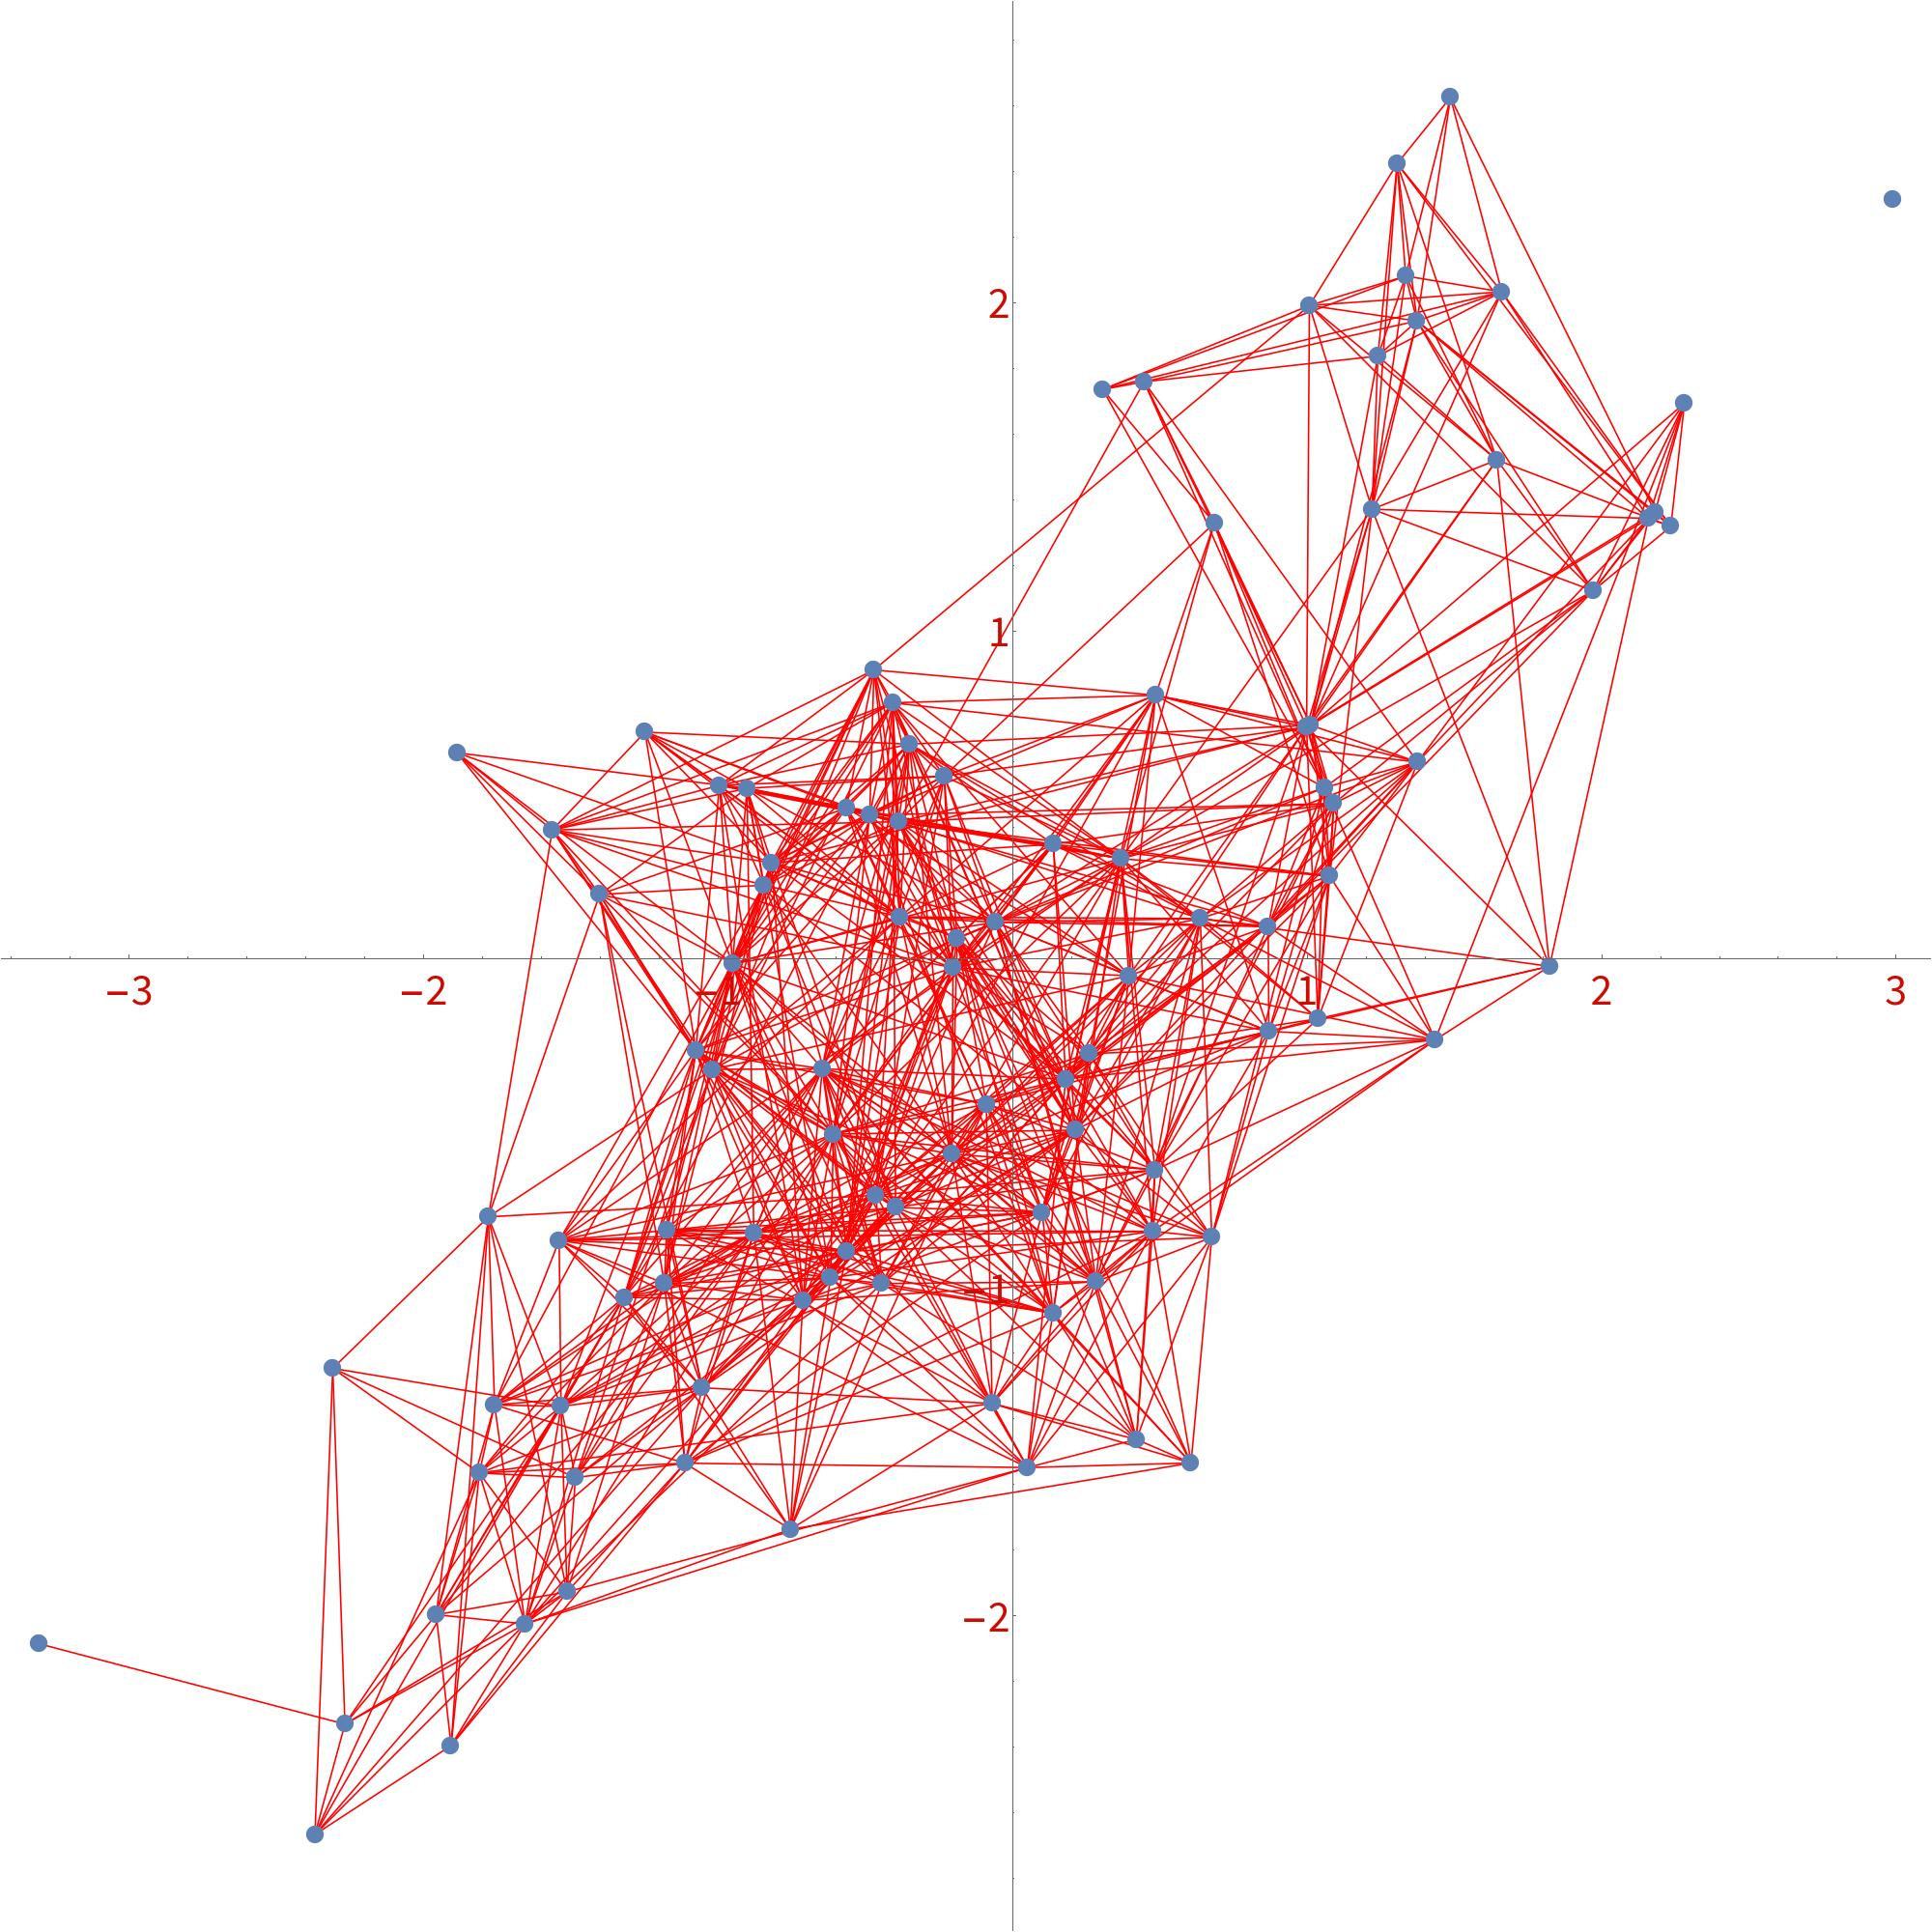
\includegraphics[width = 0.5\textwidth]{gaussian_rgg_non_spherical1.jpg}
    \caption[Gaussian non-spherical prior]{Gaussian prior with $\Sigma = \begin{pmatrix} 3 & 1.5 \\ 1.5 & 1\end{pmatrix}$}
\end{figure}

\begin{figure}
    \centering
    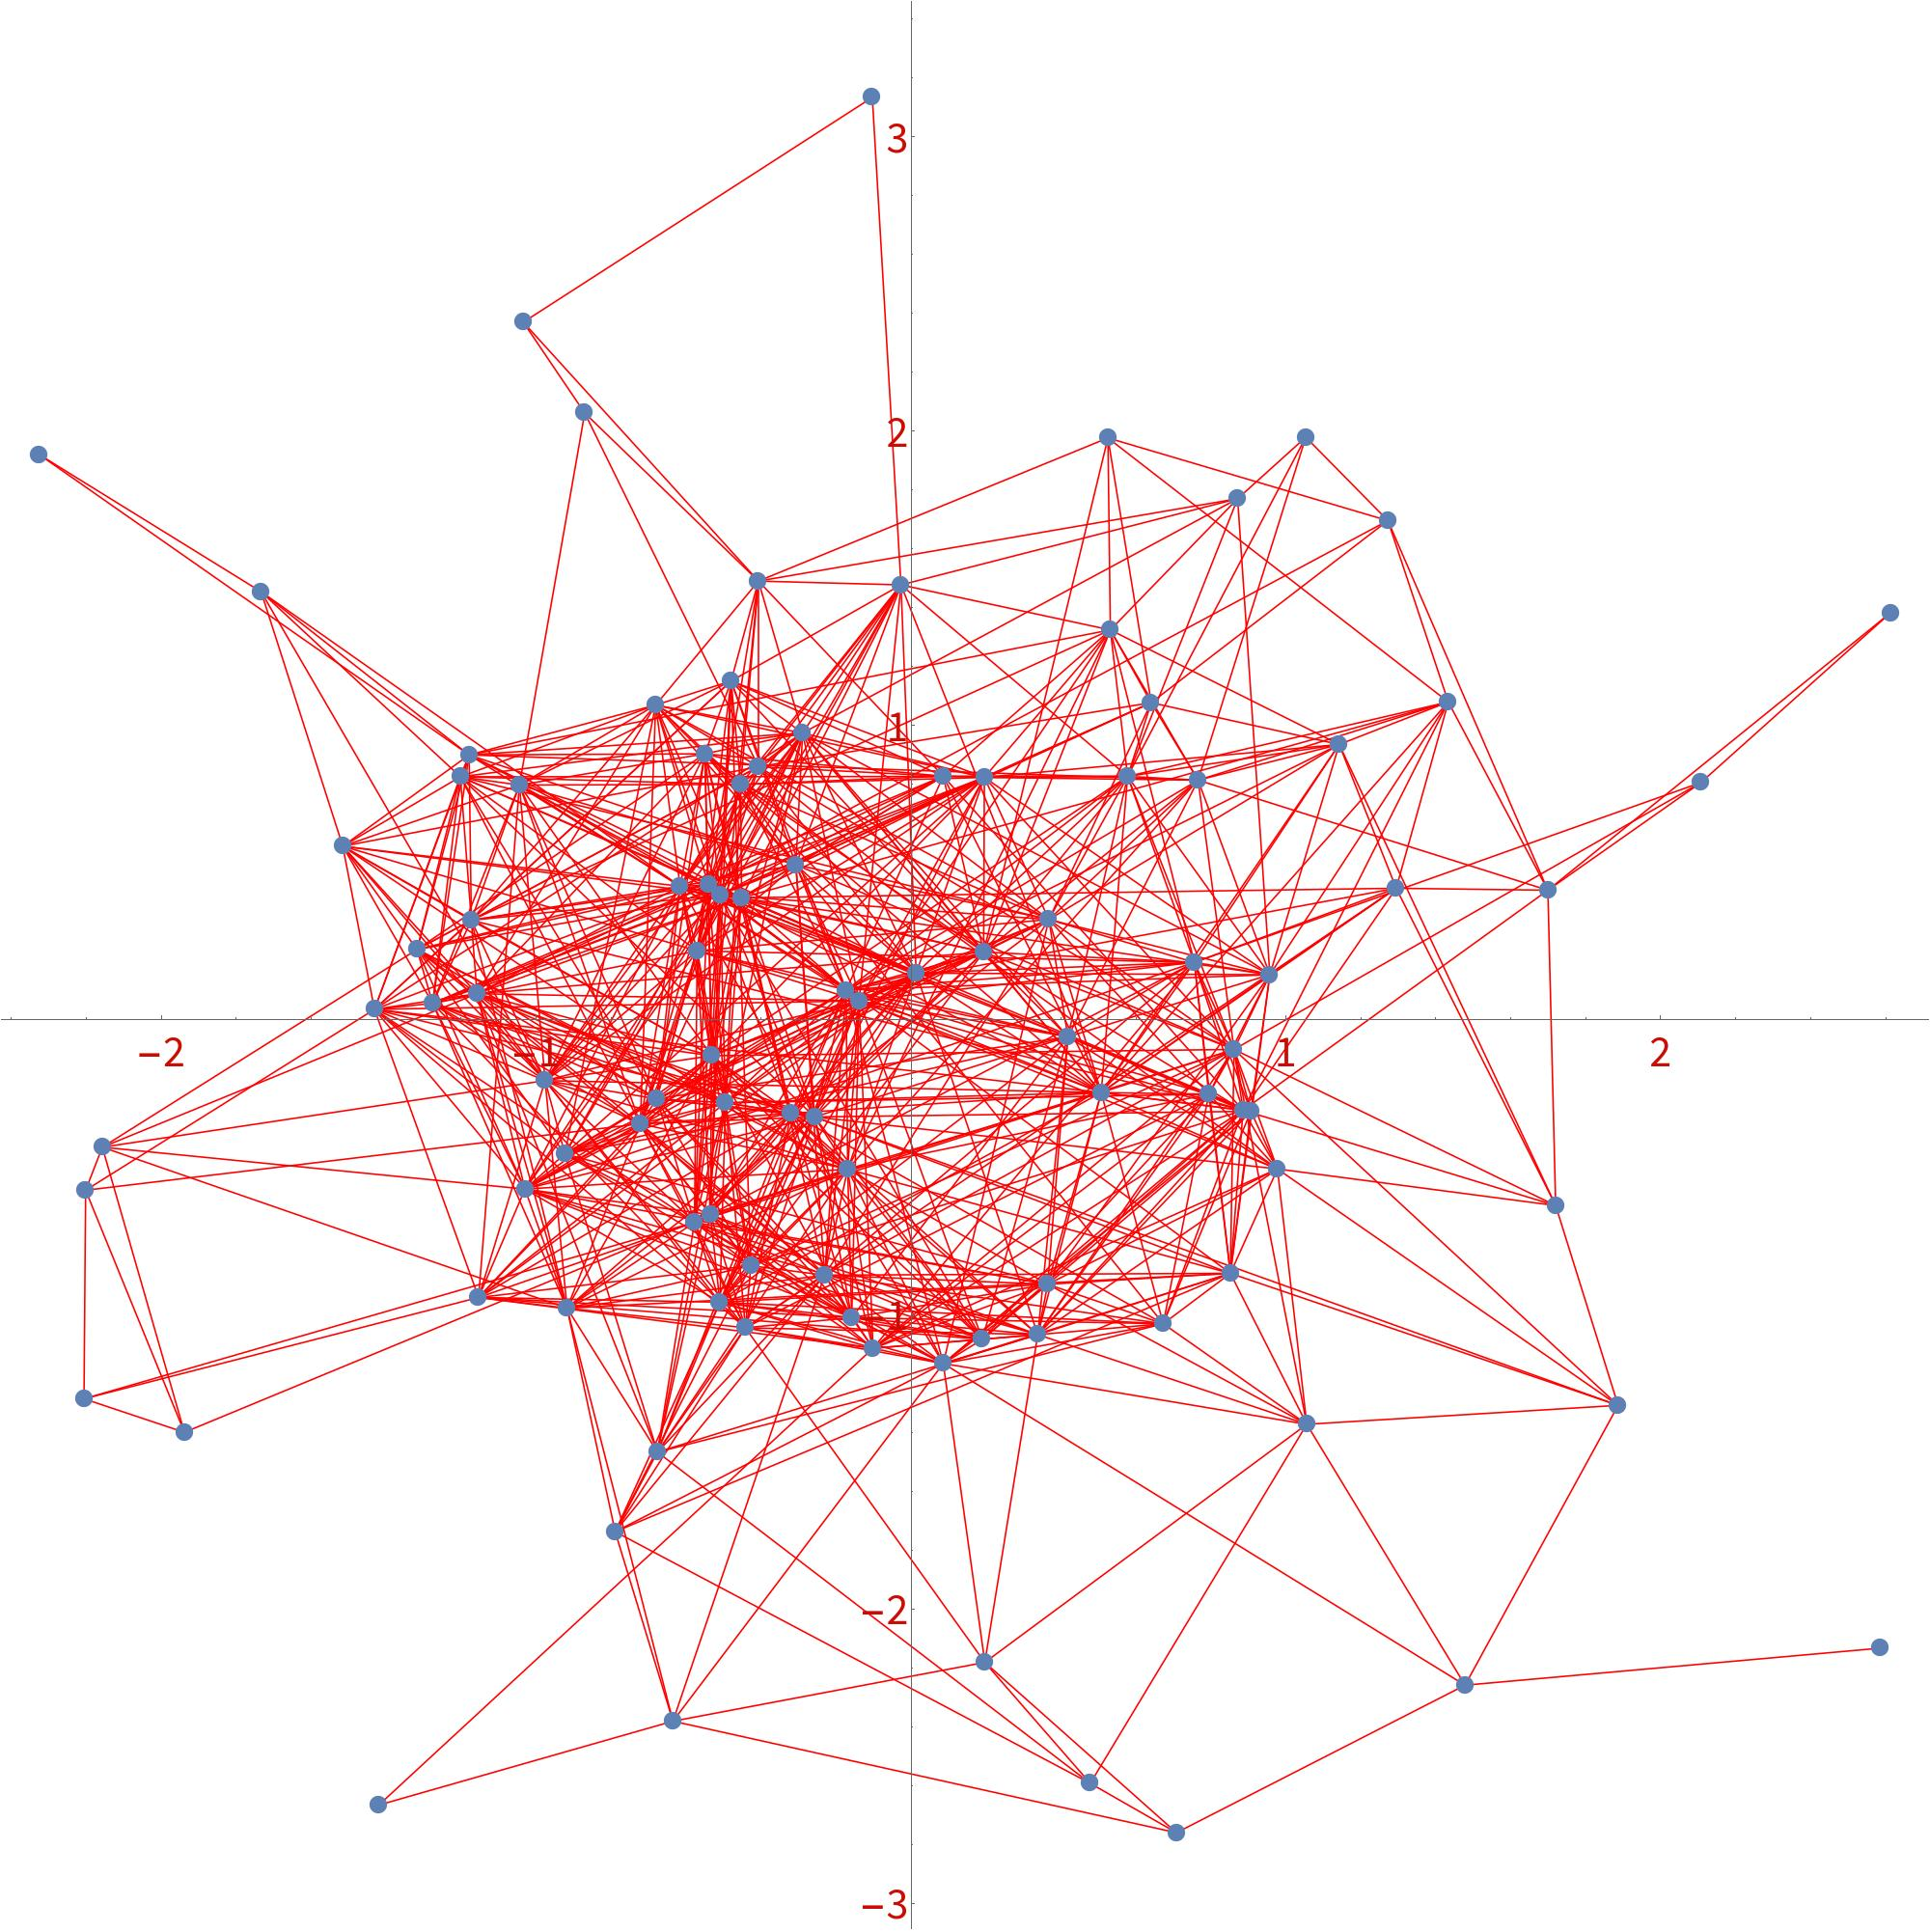
\includegraphics[width = 0.5\textwidth]{multivariatet.jpg}
    \caption[Spherical Multivariate T with 15 degrees of freedom]{Multivariate T with $\Sigma = \mc{I}$ and 15 degrees of freedom.}
\end{figure}

\printbibliography
\appendix


\chapter{Distance PDF}
\raggedright

Let
\begin{equation*}
    X_i, X_j \sim \mathcal{N}(\bs{0}, \half\sigma^2\mc{I}_n)
\end{equation*}

Then
\begin{equation*}
    Y_{ij} = X_i - X_j \sim \mathcal{N}(\bs{0}, \sigma^2\mc{I}_n)
\end{equation*}

Denoting the squared distance between $X_i$ and $X_j$ by the random variable
\begin{equation*}
    D_{ij} = Y_{ij}^TY_{ij}
\end{equation*}
we find ourselves in the context defined in Mathai, so we have that the pdf of $D_{ij}$ is
\begin{equation*}
    f(u) = \sumlim{k}{0}{\infty}(-1)^kc_k\frac{u^{\frac{n}{2}+k-1}}{\Gamma(\frac{n}{2}+k)}
\end{equation*}
where
\begin{align}
    c_0 &= \prodlim{j}{1}{n}(2\lambda_j)^{-\half} \notag\\
    c_k &= \frac{1}{k}\sumlim{r}{0}{k-1}d_{k-r}c_r,\quad k\geq1 \\
    d_k &= \half\sumlim{j}{1}{n}(2\lambda_j)^{-k},\quad k\geq1 \notag
\end{align}
with $\{\lambda_j\}$ denoting the eigenvalues of the covariance matrix of $Y_{ij}$, $\sigma^2\mathcal{I}_n$, so
\begin{equation*}
    \lambda_j = \sigma^2,\quad j\in\{1,\,\dots,\,n\}
\end{equation*}
implying
\begin{align}
    c_0 &= (2\sigma^2)^{-\frac{n}{2}} \\
    d_k &= \half\sumlim{j}{1}{n}(2\sigma^2)^{-k} \notag\\
        &= \frac{n}{2}(2\sigma^2)^{-k},\quad k\geq1
\end{align}

Assuming that $n = 2m,\,m\in\mb{N}$, we will prove by induction that
\begin{equation*}
    c_k = \comb{m + k - 1}{k}2^{-k-m}(\sigma^2)^{-m - k},\quad k \geq 0
\end{equation*}
where $\comb{a}{b}$ denotes combinations of $a$ taken $b$. For the sake of the notation, let us assume that $\comb{0}{0} = 1$. \\

From (A.2), we have that
\begin{align*}
    c_0 &= 2^{-\frac{n}{2}}(\sigma^2)^{-frac{n}{2}} \\
    &= \ub{1}_{\comb{m-1}{0}} \times 2^{-m}(\sigma^2)^{-m}
\end{align*}
so the induction hypotesis holds for $c_0$. \\

Now, assuming that the hypothesis holds for $c_j,\,j\in\{0,\,\dots,\,k-1\}$, we will prove it holds for $c_k$ as well. Let us calculate each term of (A.1).

\begin{align*}
    d_{k-r}c_r &= m2^{-k+r}(\sigma^2)^{-k+r} \times \comb{m+r-1}{r}2^{-r-m}(\sigma^2)^{-m-r} \\
    &= m\comb{m+r-1}{r} 2^{-k-m}(\sigma^2)^{-k-m} 
\end{align*}
Then
\begin{align}
    c_k &= \frac{1}{k}\sumlim{r}{0}{k-1}m\comb{m+r-1}{r} 2^{-k-m}(\sigma^2)^{-k-m} \notag\\
    &= \frac{m}{k}2^{-k-m}(\sigma^2)^{-k-m}\sumlim{r}{0}{k-1}\comb{m+r-1}{r}  \\
\end{align}
We will prove by induction over k that $\sumlim{r}{0}{k-1}\comb{m+r-1}{r} = \comb{m+k-1}{k-1}$. For $k = 1$ it obviously holds. Assuming our assumption is true for some $k$, we will prove it holds for $k+1$ as well.
\begin{align*}
    \sumlim{r}{0}{k}\comb{m+r-1}{r} &= \sumlim{r}{0}{k-1}\comb{m+r-1}{r} + \comb{m+k-1}{k} \\
    &= \comb{m+k-1}{k-1} + \comb{m+k-1}{k} \\
    &= \comb{m+k}{k}
\end{align*}
making the induction proof complete.

(A.4) then becomes
\begin{align*}
    c_k &= \frac{m}{k}\comb{m+k-1}{k-1}2^{-k-m}(\sigma^2)^{-k-m} \\
    &= \comb{m+k-1}{k}2^{-k-m}(\sigma^2)^{-k-m}
\end{align*}
so the induction is complete. We now have that
\begin{align*}
    f(u) &= \sumlim{k}{0}{\infty}(-1)^k\comb{m+k-1}{k}2^{-k-m}(\sigma^2)^{-k-m}\frac{u^{m+k-1}}{\Gamma(m+k)} \\
    &= \sumlim{k}{0}{\infty}(-1)^k\frac{(m+k-1)!}{(m-1)!k!}2^{-k-m}(\sigma^2)^{-k-m}\frac{u^{m+k-1}}{(m+k-1)!} \\
    &= \sumlim{k}{0}{\infty}(-1)^k\frac{\cancel{(m+k-1)!}}{(m-1)!k!}2^{-k-m}(\sigma^2)^{-k-m}\frac{u^{m+k-1}}{\cancel{(m+k-1)!}} \\
    &= \frac{2^{-m}(\sigma^2)^{-m}u^{m-1}}{(m-1)!}\sumlim{k}{0}{\infty}(-1)^k\frac{1}{k!}2^{-k}(\sigma^2)^{-k}u^{k} \\
    &= \frac{2^{-m}(\sigma^2)^{-m}u^{m-1}}{(m-1)!}\sumlim{k}{0}{\infty}\frac{(-(2\sigma^2)^{-1}u)^k}{k!} \\
    &= \frac{(2\sigma^2)^{-m}u^{m-1}}{(m-1)!}e^{-(2\sigma^2)^{-1}u}
\end{align*}

\chapter{Free Energy}
\begin{equation}
    \mc{F} = \left<log\mb{P}(\mc{G}\mid \bf{X})\right>_{q(\bf{X})} - KL(q(\bf{X}) \mid\mid \mb{P}(\bf{X}))
\end{equation}
\begin{align*}
    \left<log\mb{P}(\mc{G}\mid \bf{X})\right>_{q(\bf{X})} &= \int\limits_{(\mb{R}^n)^N} d\bf{X}
\end{align*}

\end{document}
